\def\inputsize{7}

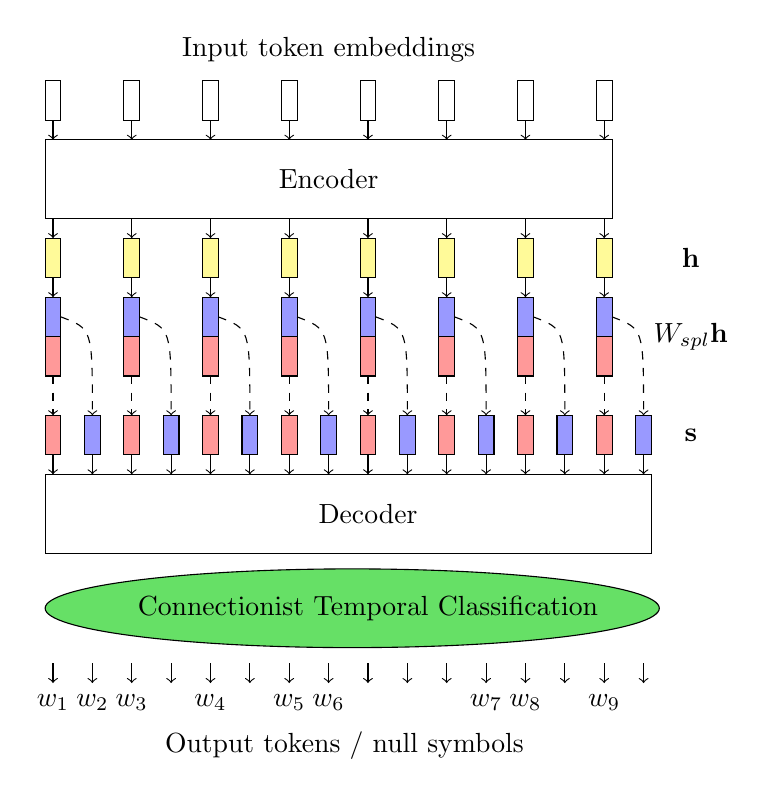
\begin{tikzpicture}[]

\draw (\inputsize / 2 + 0.1, -0.1) node {Input token embeddings};

\foreach \i in {0,...,\inputsize} {
	\draw (\i,-0.5) rectangle (\i+0.2,-1);
    \draw [->] (\i+0.1,-1) -- (\i+0.1, -1.25);
};

\draw (0, -1.25) rectangle (\inputsize + 0.2, -2.25);
\draw (\inputsize / 2 + 0.1, -1.75) node {Encoder};

\foreach \i in {0,...,\inputsize} {
	\draw [->] (\i+0.1,-2.25) -- (\i+0.1, -2.5);
    \draw[fill=yellow!40] (\i,-2.5) rectangle (\i+0.2,-3);

    \draw [->] (\i+0.1,-3) -- (\i+0.1, -3.25);
	\draw[fill=blue!40] (\i,-3.25) rectangle (\i+0.2,-3.75);
	\draw[fill=red!40] (\i,-3.75) rectangle (\i+0.2,-4.25);

    \draw [dashed,->] (\i+0.1,-4.25) -  - (\i+0.1, -4.75);
    \draw [dashed,->] (\i+0.2,-3.5) .. controls (\i + 0.6, -3.65) .. (\i+0.6, -4.75);

	\draw[fill=red!40] (\i,-4.75) rectangle (\i+0.2,-5.25);
	\draw[fill=blue!40] (\i + 0.5,-4.75) rectangle (\i+0.7,-5.25);

    \draw [->] (\i+0.1,-5.25) - - (\i+0.1, -5.5);
    \draw [->] (\i+0.6,-5.25) - - (\i+0.6, -5.5);
};

\draw (\inputsize + 1.2, -2.75) node {$\mathbf{h}$};
\draw (\inputsize + 1.2, -3.75) node {$W_{\text{spl}}\mathbf{h}$};
\draw (\inputsize + 1.2, -5.00) node {$\mathbf{s}$};

\draw (0, -5.5) rectangle (\inputsize + 0.7, -6.5);
\draw (\inputsize / 2 + 0.5 + 0.1, -6.0) node {Decoder};

\draw [fill=green!80!black!60] (\inputsize / 2 + 0.4,-7.2) circle [x radius=\inputsize / 2 + 0.4, y radius=0.5];
\draw (\inputsize / 2 + 0.6, -7.2) node {Connectionist Temporal Classification};

\foreach \i in {0,...,\inputsize} {
   \draw [->] (\i+0.1,-7.9) - - (\i+0.1, -8.15);
   \draw [->] (\i+0.6,-7.9) - - (\i+0.6, -8.15);
}

\draw  (0+0.1,-8.4) node {$w_1$};
\draw  (0+0.6,-8.4) node {$w_2$};
\draw  (1+0.1,-8.4) node {$w_3$};
\draw  (1+0.6,-8.4) node {$\varnothing$};
\draw  (2+0.1,-8.4) node {$w_4$};
\draw  (2+0.6,-8.4) node {$\varnothing$};
\draw  (3+0.1,-8.4) node {$w_5$};
\draw  (3+0.6,-8.4) node {$w_6$};
\draw  (4+0.1,-8.4) node {$\varnothing$};
\draw  (4+0.6,-8.4) node {$\varnothing$};
\draw  (5+0.1,-8.4) node {$\varnothing$};
\draw  (5+0.6,-8.4) node {$w_7$};
\draw  (6+0.1,-8.4) node {$w_8$};
\draw  (6+0.6,-8.4) node {$\varnothing$};
\draw  (7+0.1,-8.4) node {$w_9$};
\draw  (7+0.6,-8.4) node {$\varnothing$};

\draw (\inputsize / 2 + 0.3, -8.95) node {Output tokens / null symbols};

\end{tikzpicture}